\documentclass[11pt]{amsart}
\usepackage{amssymb}
\usepackage{mathtools,color}
\usepackage[alphabetic]{amsrefs}
\usepackage{leftidx}
\usepackage{subcaption}
\usepackage{tikz}
\usepackage{eucal}
\usepackage{fullpage}
\setlength{\footskip}{30pt}

\newcommand{\T}{\mathcal{T}}
\renewcommand{\emptyset}{\text{\O}}
\newcommand{\f}{\mathbf{f}}
\newcommand{\jk}[1]{\textcolor{red}{[Jan: #1]}}
\newcommand{\CC}{\ensuremath{\mathcal{C}}}
\newcommand{\N}{\mathbb{N}}
\newcommand{\la}{\lambda}
\renewcommand{\SS}{\mathbf{S}}
\DeclareMathOperator{\EMD}{EMD}

\theoremstyle{plain}
\newtheorem{theorem}{Theorem}[section]
\newtheorem{prop}[theorem]{Proposition}
\newtheorem{lemma}[theorem]{Lemma}
\newtheorem{corollary}[theorem]{Corollary}

\theoremstyle{remark}
\newtheorem{rem}[theorem]{Remark}

\newcommand{\question}[1]{\textcolor{blue}{\textbf{#1}}}



\begin{document}

\title{The sum of all width-1 contingency tables}

\author{William Q. Erickson}
\address{
William Q.~Erickson\\
Department of Mathematics\\
Baylor University \\ 
One Bear Place \#97328\\
Waco, TX 76798} 
\email{Will\_Erickson@baylor.edu}

\author{Jan Kretschmann}
\address{
Jan Kretschmann\\
Department of Mathematical Sciences\\
University of Wisconsin--Milwaukee \\ 
3200 N.~Cramer St.\\
Milwaukee, WI 53211} 
\email{kretsc23@uwm.edu}

\begin{abstract}
We say that a square nonnegative integer matrix has width 1 if its nonzero entries lie along a path consisting of steps to the south and to the east. 
In particular, in optimal transport theory, the output of the northwest corner rule is necessarily a contingency table of width 1.
Therefore, in seeking to streamline and to generalize existing methods for computing the mean earth mover's distance between pairs of discrete histograms, we realized that the problem can be reduced to finding an explicit formula for the sum of all width-1 contingency tables (with given dimensions and grand sum).
Our main result is a formula for this sum, obtained by studying the order complexes of products of chains $[i] \times [j]$.
We also give an alternative formula, which is less transparent but computationally more efficient, obtained from the perspective of Stanley--Reisner theory by viewing the desired matrix sum as a product of monomials.
\end{abstract}

\subjclass[2020]{Primary 05E45; Secondary 13F55, 05B20}

\keywords{Simplicial complexes, order complex, Stanley--Reisner rings, Stanley decompositions, optimal transport, earth mover's distance}


\maketitle


\section{Introduction}

Let $\T(d,n)$ be the set of all $n \times n$ matrices with nonnegative integer entries summing to $d$, such that the nonzero entries lie along a single path consisting of steps to the south and to the east.  
We call these \emph{width-1} matrices, since their support has width 1 in the underlying poset of matrix coordinates; 
moreover, they are the exponent matrices of width-1 monomials, in the language of Sturmfels~\cite{Sturmfels}*{p.~138}.
In this paper, we solve the problem of writing down an explicit formula for the sum $\SS(d,n)$ of all matrices in $\T(d,n)$. 
The motivation for this problem actually arose from optimal transport theory: we were seeking an explicit formula for the mean of the discrete earth mover's distance (EMD) on pairs of histograms with $d$ data points in $n$ bins.  
Our solution, however, is obtained via combinatorial techniques in abstract simplicial complexes and Stanley--Reisner theory.

The EMD is a metric on a space of histograms, and can be viewed as the solution to the founding problem of optimal transport theory.  
This explains our notation ``$\T$,'' in fact, which stands for ``transport matrix.''
Since its 18th-century origin in the earth-moving problem posed by Gaspard Monge~\cite{monge}, and its modern re-popularization by Rubner et.\ al.\ \cite{rubner} in computer vision, the EMD has proven to be a powerful tool in applications such as physics \cite{komiske}, cosmology \cite{frisch}, political science \cite{lupu}, epidemiology \cite{melnyk}, and many others; see~\cite{Villani} for a comprehensive treatment.  
In \cite{BW}, Bourn and Willenbring derived a recursive formula to compute the mean value of the EMD, in the context of one-dimensional histograms with bins located at consecutive points $1, \ldots, n$ on the number line. 
In this case the cost of transport between two bins is the $\ell_1$-distance between them.  
The recursion in~\cite{BW} was obtained by means of a clever application of the Robinson--Schensted--Knuth (RSK) correspondence and manipulations with generating functions.  
The paper~\cite{FV} then took an analytical approach to close the recursion in the setting of probability distributions rather than discrete histograms.
Each author of the present paper has worked independently to generalize the results of~\cite{BW} in different directions \cites{EricksonAStat, KretschmannMasters, KretschmannPhD}, which led us to seek an explicit, non-recursive formula for the mean EMD on discrete histogram pairs.

In Section~\ref{sec:EMD}, we describe how this motivating problem can be reduced to the main problem stated above, namely, finding the sum $\SS(d,n)$ of all matrices in $\T(d,n)$.  
To summarize, there is a well-known algorithm in the transport theory literature known as the ``northwest corner rule,'' which associates each histogram pair to a unique contingency table $T \in \T(d,n)$, also known as a \emph{transport matrix}. 
This output $T$, by the nature of the northwest corner rule, necessarily has width 1. 
For a certain class of matrices $C$ defining the cost of transport between bins, the EMD can be realized as the trace of the matrix product $C^\mathsf{T} T$. 
By exploiting the linearity of the trace, we can realize the sum of all EMD's as the trace of a single matrix product, namely $C^\mathsf{T} \cdot \SS(d,n)$. 
This not only furnishes an explicit formula for the mean EMD, but also dramatically increases flexibility: 
whereas the recursive methods above have focused on one-dimensional histograms with cost given by $\ell_1$-distance, our method of first finding the sum of all transport matrices allows us to independently vary the cost matrix $C$.  
In fact, our result immediately yields the mean EMD for \emph{any} cost matrix $C$ that has the Monge property, defined below in ~\eqref{Monge property}.

In Section~\ref{sec:ASC}, we translate the problem of finding $\SS(d,n)$ into the language of abstract simplicial complexes.  
The set of matrix coordinates forms a poset under the product order, and the support of a width-1 matrix is a chain in this poset.  
The set of all chains is called the \emph{order complex}, and its $f$-vector counts the number of chains of each size.  
We obtain the $f$-vector by way of the $h$-vector, where our primary tool is the shelling described in the paper~\cite{BCS} by Billera--Cushman--Sanders on the Stanley decomposition of the harmonic oscillator.  
Armed with these combinatorial data, in Theorem~\ref{thm:main result} we record our main result, an explicit formula for the desired sum $\SS(d,n)$ of width-1 matrices.  By way of preview, we include this formula below:
\[
\SS(d,n)_{ij} = \sum_{\ell=1}^{\min\{d, \: 2n-1\}} \binom{d}{\ell} \cdot [t^{\ell-1}] g_{ij} \overline{g}_{ij},
\]
where the $[t^{\ell-1}]$ extracts a single coefficient from the product of two polynomials; it will turn out that $g_{ij}(t)$ and $\overline{g}_{ij}(t)$ are combinations of certain $f$-polynomials of order complexes.

Finally, in Section~\ref{sec:WillFormula}, we present an alternative formula for $\SS(d,n)$ by taking an approach from combinatorial commutative algebra.  
In particular, we shift perspective to the problem of finding the product of all monomials in the $d$th graded component of the Stanley--Reisner ring of the order complex.  
Although the argument and the final formula (Theorem~\ref{thm:main result h polys}) in this section are less transparent than those in Section~\ref{sec:JanFormula}, this alternative formula is significantly faster for computations.

\section{Statement and motivation of the problem}
\label{sec:EMD}

\subsection{Statement of the problem} 
For positive integers $i$ and $j$, we define the following poset, equipped with the product order $\preceq$:
\begin{equation}
    \label{def:Pi}
    \Pi_{ij} \coloneqq \{(x,y) : 1 \leq x \leq i, \: 1 \leq y \leq j\}, \qquad
    (x,y) \preceq (x',y') \iff x \leq x' \text{ and } y \leq y'.
\end{equation}
Elsewhere in the literature, $\Pi_{ij}$ is sometimes written as $[i] \times [j]$.
We will abbreviate $\Pi_n \coloneqq \Pi_{nn}$.  
Because our main problem deals with $n \times n$ matrices, we will always be working inside $\Pi_{n}$, but it will be useful to consider its subposets $\Pi_{ij}$, which are the lower-order ideals generated by each matrix position $(i,j)$. 
This is the reason we are using $i$ and $j$ as the matrix dimensions, rather than as the matrix coordinates (which we label $x$ and $y$).

We adopt the standard terminology from order theory: in particular, a \emph{chain} is a totally ordered subset of $\Pi_{ij}$, and an \emph{antichain} is a subset whose elements are pairwise incomparable. 
The \emph{width} of a subset $S \subseteq \Pi_{ij}$ is the size of the largest antichain contained in $S$. 
Equivalently, by Dilworth's theorem, the width of $S$ equals the minimum number of chains into which $S$ can be partitioned.  

We define the \emph{support} of an $i \times j$ matrix $M$ as follows:
\[
\operatorname{supp}(M) \coloneqq \{(x,y) \in \Pi_{ij} : M_{xy} \neq 0\}.
\]
We will say that $M$ is a \emph{width-1} matrix if $\operatorname{supp}(M) \subseteq \Pi_{ij}$ has width 1.  
Note that when $\Pi_{ij}$ is visualized as the coordinates of an $i \times j$ matrix, the relation $\preceq$ means ``weakly northwest''; therefore, in a width-1 matrix, all nonzero entries lie along a path from the northwest to the southeast corner (i.e., a maximal chain), consisting of steps to the south and to the east. 
Now let ${\rm M}_n(\N)$ denote the set of $n \times n$ matrices with entries in $\N = \{0, 1, 2, \ldots\}$. For a positive integer $d$, we define the set
\begin{equation}
    \label{T(d,n) definition}
    \T(d,n) \coloneqq \{ T \in {\rm M}_n(\N) : \text{$T$ is width-1 and $\sum_{i,j} T_{ij} = d$}\}.
\end{equation}
(As mentioned above, the ``$\T$'' and ``$T$'' stand for ``transport matrix,'' to  be explained below.)  The main problem of this paper is to write down an explicit formula for the sum of all these matrices, which we call
\begin{equation}
    \label{Bold T definition}
    \SS(d,n) \coloneqq \sum_{\mathclap{T \in \T(d,n)}} T.
\end{equation}

\subsection{Motivation: the earth mover's distance}

Our motivation behind finding an explicit formula for $\SS(d,n)$ was to be able to compute, as efficiently as possible, the mean of the \emph{earth mover's distance} (EMD), taken over all pairs of histograms with $d$ data points and $n$ bins. 
We now proceed to explain the EMD, and then we show in Proposition~\ref{prop:EMD=tr(CS)} how $\SS(d,n)$ is the key to finding an explicit formula for the mean EMD.  
(This subsection may, however, be omitted without loss of continuity in solving the main problem of this paper.)

Let $\CC(d,n)$ denote the set of weak integer compositions of $d$ into $n$ parts; we write an element of $\CC(d, n)$ as $\la = (\la_1, \ldots, \la_n)$, where each $\la_i \in \N$ and $\sum_i \la_i = d$.  
It is well known that $\#\CC(d,n) = \binom{d+n-1}{d}$.
Elements of $\CC(d,n)$ can be viewed as histograms with $d$ data points and with bins $1, \ldots, n$, by taking $\la_i$ to be the number of data points in bin $i$.  
We will thus speak interchangeably of ``compositions'' and ``histograms.''  

Intuitively, given two histograms $\lambda,\mu \in \CC(d,n)$, their earth mover's distance $\EMD(\la,\mu)$ is the minimum amount of work required to transform $\la$ into $\mu$.  
In order to make precise the notion of ``work,'' we must first specify an $n \times n$ matrix $C = [C_{ij}]$, where $C_{ij} \geq 0$ is the \emph{cost} of transporting one data point from bin $i$ to bin $j$.  
(The cost is also called ``ground distance'' in the literature.)
The EMD is defined in \cite{rubner} by the solution to a certain linear programming problem (typically named after Gaspard Monge \cite{monge}, or various combinations of Monge, Kantorovich, Hitchcock, and Koopman).  
In particular, we want to find a real $n \times n$ matrix $T = [T_{ij}]$ in order to solve the following \emph{Monge problem}:
\begin{align}
    \text{Minimize} \quad & \sum_{\mathclap{i,j=1}}^n C_{ij} T_{ij}, \label{work}\\
    \text{subject to} \quad & T_{ij} \geq 0 & \text{for all } 1 \leq i,j \leq n, \label{nonneg}\\
    \text{and} \quad & \sum_{j=1}^n T_{ij} = \la_i & \text{for each }1\leq i \leq n, \label{rows}\\
    \text{and} \quad & \sum_{i=1}^n T_{ij} = \mu_j & \text{for each } 1 \leq j \leq n. \label{cols}
\end{align}
The matrix $T$ is typically called a \emph{transport matrix}, a \emph{transport plan}, or a \emph{flow matrix} in the literature.  
One can regard $T$ as a contingency table with $\la$ and $\mu$ as its margins.  
The idea is that any such $T$ encodes a way to transform $\la$ into $\mu$, at the expense of the work calculated in~\eqref{work}: 
namely, $T_{ij}$ equals the number of data points inside $\la$ that must be transported from bin $i$ to bin $j$.  
Hence \eqref{nonneg} any candidate $T$ must have nonnegative entries; \eqref{rows} the $i$th row sum (i.e., number of data points transported out of bin $i$) must equal the number of data points in bin $i$ of $\la$; 
likewise, \eqref{cols} the $j$th column sum (the number of data points transported into bin $j$) must equal the number of data points in bin $j$ of $\mu$.  

Let $\T_{\la\mu}$ be the set of all transport matrices $T$ satisfying constraints \eqref{nonneg}--\eqref{cols}.
Once we have found an optimal solution $T$ to the Monge problem, the \emph{earth mover's distance} (EMD) is defined to be the objective quantity in \eqref{work}.  In other words,
\[
    \EMD(\la,\mu) \coloneqq \inf_{T \in \T_{\la\mu}} \left\{\sum_{i,j} C_{ij} T_{ij}\right\}.
\]
By definition, then, computing the EMD depends upon first solving the Monge problem \eqref{work}--\eqref{cols}.  

The solution is nicest, in a sense, when the cost matrix $C$ has what is known as the \emph{Monge property}: 
\begin{equation}
    \label{Monge property}
    C_{ij} + C_{IJ} \leq C_{Ij} + C_{iJ}, \quad \text{for all $i<I$ and $j < J$.}
\end{equation}
The significance of the Monge property lies in a result of Hoffman \cite{hoffman}: 
namely, the Monge problem can be solved via a certain $O(2n)$-time greedy algorithm (the ``northwest corner rule''), if and only if the associated cost matrix $C$ has the Monge property.  
The northwest corner rule solves the Monge problem by constructing an optimal transport matrix $T \in \mathcal T_{\la\mu}$: 
beginning in the upper-left, the algorithm sets $T_{11} = \min\{\la_1,\mu_1\}$, and then modifies both $\la_1$ and $\mu_1$ by subtracting $T_{11}$ (so at least one of them becomes 0).  
This allows us to fill the remainder of either the first row or the first column with 0's;
then we proceed either south or east, and repeat the process until we have filled the entire matrix $T$, which is the solution to the Monge problem. 

It is immediate from this construction that $T$ has nonnegative integer entries summing to $d$, and has row and column sums given by $\la$ and $\mu$, respectively.  
Moreover, the very nature of the northwest corner rule forces the nonzero entries of $T$ to lie in a single path traveling either south or east at each step: 
in other words, $T$ is width-1 and hence $T \in \T(d,n)$, as defined in~\eqref{T(d,n) definition}. 
Therefore, writing $T_{\la\mu}$ for the output of the northwest corner rule applied to the pair $(\la,\mu$), we have a bijection
\begin{align}
\label{bijection histogram pairs CTs}
\begin{split}
 \CC(d, n) \times \CC(d,n) &\xrightarrow{\phantom{\text{NW corner rule}}}\T(d,n),\\
 (\la,\mu) &\xmapsto{\text{NW corner rule}} T_{\la\mu}.
 \end{split}
\end{align}
(To see that this correspondence is surjective, one can appeal to the Robinson--Schensted--Knuth correspondence, where each element of $\CC(d,n)$ is viewed as the weakly increasing sequence $1^{\la_1}\!\ldots n^{\la_n}$.  
This is the approach taken by~\cite{BW}.)

We conclude this section with a proposition explaining the significance of the sum $\SS(d,n)$ of all matrices in $\T(d,n)$:

\begin{prop}
    \label{prop:EMD=tr(CS)}
    Let $C$ be an $n \times n$ matrix with the Monge property.
    Then the mean EMD on $\CC(d,n) \times \CC(d,n)$ equals
    \[
    \frac{1}{\binom{d+n-1}{d}^2} \cdot \operatorname{tr}\!\Big(C^\mathsf{T}\! \cdot \SS(d,n)\Big).
    \]
    \end{prop}

\begin{proof}

To obtain the mean, we multiply the reciprocal of $\#\CC(d,n)^2 = \binom{d+n-1}{d}^2$ by the following sum, which we rewrite using the linearity of the trace:
\begin{align*}
    \sum_{\mathclap{\substack{(\la,\mu) \\ \in \CC(d,n) \times \CC(d,n)}}} \EMD(\la,\mu) &= \sum_{(\la,\mu)} \sum_{i,j=1}^n C_{ij}(T_{\la\mu})_{ij}\\
    &= \sum_{(\la,\mu)} \operatorname{tr}(C^\mathsf{T}  T_{\la\mu})\\
    &= \operatorname{tr}\left(C^\mathsf{T} \! \cdot \sum_{(\la,\mu)} T_{\la\mu}\right)\\
    &= \operatorname{tr}\left(C^\mathsf{T} \! \cdot \sum_{\mathclap{T \in \T(d,n)}} T\right)\\
    &= \operatorname{tr}\Big(C^\mathsf{T} \! \cdot \SS(d,n)\Big),
\end{align*}
where the last two equalities follow from \eqref{bijection histogram pairs CTs} and \eqref{T(d,n) definition}, respectively.
\end{proof}

Hence if we had an explicit formula for $\SS(d,n)$, then we could compute the mean EMD by taking the trace of a single matrix product.  
This would be not only more direct, but also much more flexible than existing methods, in that we could study the EMD with respect to any cost matrix $C$ with the Monge property.  
We devote the rest of the paper to deriving an explicit formula (two, in fact: see Theorems~\ref{thm:main result} and~\ref{thm:main result h polys}).

\section{Simplicial complexes}
\label{sec:ASC}

Solving our problem requires one to consider an arbitrary matrix coordinate $(i,j)$ and determine the contribution of each matrix in $\T(d,n)$ to the $(i,j)$ entry in $\SS(d,n)$.
Our approach draws from the theory of abstract simplicial complexes.  
Throughout this section, we largely follow the exposition in~\cite{StanleyAC}*{Ch.~12}; see also~\cite{24Hours}*{Ch.~16}.  We outline the general theory in the first subsection, before adapting it to our main problem in the second.
 
 \subsection{Abstract simpicial complexes}
 \label{sub:simplicial complexes}

 Given a finite set $V$, an \emph{(abstract) simplicial complex} on $V$ is a collection $\Delta$ of subsets of $V$ such that
 \begin{itemize}
     \item $\{v\} \in \Delta$ for all $v \in V$;
     \item if $S \in \Delta$ and $R \subseteq S$, then $R \in \Delta$.
 \end{itemize}
 Elements of $V$ are called \emph{vertices}, and $V$ is called the \emph{vertex set}.  The elements of $\Delta$ are called \emph{faces}, and the \emph{dimension} of a face is one less than its cardinality.  The dimension of $\Delta$ is the maximum of the dimensions of its faces.  
 
 Let $\Delta$ be a nonempty simplicial complex of dimension $m-1$. 
We denote by $f_i$ the number of faces of dimension $i$.  In particular, $f_{-1} = 1$ since $\emptyset \in \Delta$.  The \emph{$f$-vector} is the sequence $(f_0, \ldots, f_{m-1})$, and the \emph{$f$-polynomial} is the (shifted) generating function of the $f$-vector:
\begin{equation}
    \label{f-poly definition}
    f(t) \coloneqq \sum_{i=0}^{m} f_{i-1} t^i = \sum_{S \in \Delta} t^{\#S}.
\end{equation}
(We deliberately choose this convention over the alternative definition $f(t) = \sum_i f_{i-1} t^{m-i}$ where the coefficients are written in decreasing order.)
It is often more convenient to work instead with the \emph{$h$-vector} $(h_0, \ldots, h_m)$, where the numbers $h_k$ are defined as follows:
\[
h(t) \coloneqq \sum_{i=0}^m h_k t^k = \sum_{i=0}^m f_{i-1} t^i (1-t)^{d-i}.
\]
We call $h(t)$ the \emph{$h$-polynomial} of $\Delta$.
We will make use of the following well-known description~\cite{24Hours}*{Lemma~16.19} of the $f$-vector as a weighted sum of the $h_k$:
\begin{equation}
    \label{h-vec to f-vec}
    f_{i-1} = \sum_{k = 0}^i \binom{m - k}{i - k} h_{k}.
\end{equation}
 Equivalently, at the level of polynomials, one can write $f(t) = (1+t)^m h(\frac{t}{1+t})$.
 
A maximal face in $\Delta$ (with respect to inclusion) is called a \emph{facet}. 
We say that $\Delta$ is \emph{pure} if every facet has the same dimension.  
A pure simplicial complex is said to be \emph{shellable} if there exists an ordering $F_1, \ldots, F_{s}$ of its facets with the following property: for all $i = 1, \ldots, s$, the power set of $F_i$ has a unique minimal element ${\rm R}(F_i)$ not belonging to the subcomplex generated by $F_1, \ldots, F_{i-1}$.  
Such an ordering is called a \emph{shelling}, and ${\rm R}(F_i)$ is called the \emph{restriction} of the facet $F_i$.  
(Elsewhere in the literature, the restriction is called the ``minimal face,'' ``minimal non-face,'' or ``separator'' of a facet.)
Crucial to our method is the following combinatorial description of the $h$-polynomial: if $F_1, \ldots, F_s$ is a shelling of $\Delta$, then we have
\[
    h(t) = \sum_{i=1}^s t^{\#{\rm R}(F_i)}.
\]
In other words, $h_k$ counts the number of facets whose restrictions have size $k$:
\begin{equation}
    \label{h-vec as restrictions}
    h_k = \#\{i : \#{\rm R}(F_i) = k\}.
\end{equation}

\subsection{The order complex of $\Pi_{ij}$}
\label{sub:order complex}

We now apply the general theory above to the main problem of this paper, i.e., writing down a formula for the matrix $\SS(d,n)$.  
Recall the poset $\Pi_{ij}$ defined in~\eqref{def:Pi}.  
We define the \emph{order complex} $\Delta_{ij}$ on $\Pi_{ij}$, such that the faces of $\Delta_{ij}$ are the chains in $\Pi_{ij}$.  
Then the facets of $\Delta_{ij}$ are the maximal chains $\{(1,1), \ldots, (i,j)\}$, all of which have size $i+j-1$; hence $\Delta_{ij}$ is pure.  
Note that each facet can be visualized as a path from the northwest to the southeast corner of an $i \times j$ matrix, consisting of steps to the south and to the east; see Figure~\ref{fig:path example}.  

\begin{figure}[ht]
    \centering
    \tikzset{every picture/.style={scale=.55}}
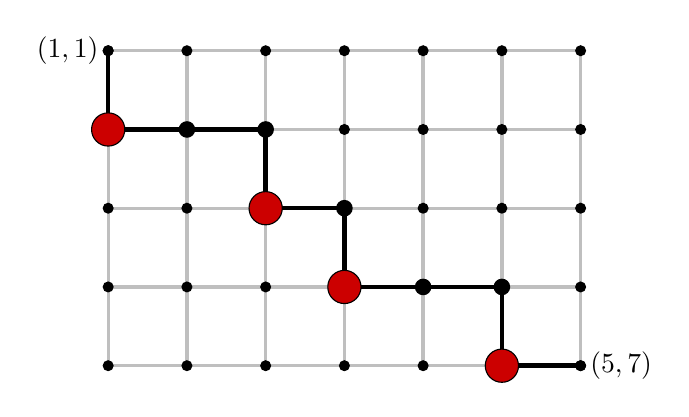
\begin{tikzpicture}
\draw[gray!50, very thick] (0,0) grid (6,4);
\foreach \i in {0,...,6}
    \foreach \j in {0,...,4}
        \fill (\i,\j) circle (2pt);
\draw[ultra thick] (0,4) -- (0,3)--(2,3)--(2,2)--(3,2)--(3,1)--(5,1)--(5,0)--(6,0) ;
\fill[black]  
(1,3) circle (3pt)
(2,3) circle (3pt)
(2,2) circle (3pt) 
(3,2) circle (3pt) 
(3,1) circle (3pt) 
(4,1) circle (3pt) 
(5,1) circle (3pt) 
(5,0) circle (3pt);

\path [draw=black, fill=red!80!black]
(0,3) circle (6pt) 
(2,2) circle (6pt)
(3,1) circle (6pt)
(5,0) circle (6pt);           
\fill[black] 
(0,4) circle (2pt) node[left] {$(1,1)$} 
(6,0) circle (2pt) node[right] {$(5,7)$};
\end{tikzpicture}
    \caption{Example of a facet $F$ of $\Delta_{5,7}$, or equivalently, a maximal chain in $\Pi_{5,7}$.  The four red circles (the \emph{corners} of $F$) indicate the restriction ${\rm R}(F)$.  This facet thus contributes $t^4$ to the polynomial $h_{5,7}(t)$.}
    \label{fig:path example}
\end{figure}

Since $\Pi_{ij}$ is a finite planar distributive lattice, it follows from~\cite{Bjorner}*{Thm.~7.1} that $\Pi_{ij}$ is shellable. 
Moreover, there exists a shelling in which the restriction ${\rm R}(F)$ of each facet $F$ is the set of its south--east \emph{corners}:
\begin{equation}
    \label{corners}
    {\rm R}(F) = \{ (x,y) \in F : \text{both $(x-1,\: y) \in F$ and $(x,\: y+1) \in F$}\}.
\end{equation}
(See~\cite{BCS}*{\S3} for details.)  In other words, a corner occurs at each \scalebox{2}{$\llcorner$}-pattern in the path representing a facet.  
It follows that given any two corners of $F$, one lies strictly northwest of the other; moreover, if $(x,y)$ is a corner of a facet of $\Pi_{ij}$, then we must have $2 \leq x\leq i$ and $1 \leq y \leq j-1$. 
Note also that ${\rm R}(F)$ fully determines $F$.
It is clear that for all facets $F$, we must have $\#{\rm R}(F) \leq \min\{i,j\}-1$, where this upper bound is attained by the facet $F$ such that ${\rm R}(F)$ contains all ``sub-diagonal'' elements of the form $(y+1,y)$.  

 To clarify that we are working in $\Delta_{ij}$, we will decorate the $f$- and $h$-vectors with superscripts (since the subscripts are already occupied):
 \[
 \text{$f$-vector:} \quad (f^{ij}_0, \ldots, f^{ij}_{i+j-2}), 
 \qquad 
 \text{$h$-vector:} \quad (h^{ij}_0, \ldots, h^{ij}_{\min\{i,j\}-1}).
 \]
 In practice, however, we will almost always work with the $f$- and $h$-polynomials, which we decorate with subscripts, as is more natural:
 \[
\text{$f$-polynomial:} \quad f_{ij} \coloneqq f_{ij}(t) = \sum_{\ell} f^{ij}_{\ell - 1} t^{\ell},
\qquad
\text{$h$-polynomial:} \quad h_{ij} \coloneqq h_{ij}(t) = \sum_{k} h^{ij}_k t^k.
 \]
 The following interpretations follow from~\eqref{f-poly definition} and~\eqref{h-vec as restrictions}, respectively.  As is standard, we write $[t^\ell]$ to the left of a polynomial to denote the coefficient of $t^\ell$ therein:
\begin{align}
        f^{ij}_{\ell - 1} &= [t^\ell] f_{ij} = \text{\# chains in $\Pi_{ij}$ of size $\ell$}, \label{coefficient f-poly}\\
        h^{ij}_k &= [t^k] h_{ij} = \text{\# maximal paths in $\Pi_{ij}$ with $k$ corners}.\label{coefficient h-poly}
\end{align}
The characterization above makes it easy to write down the $h$-vector of $\Delta_{ij}$:

\begin{prop}[\cite{MacMahon}]
    \label{prop:h-vec}
    We have $h^{ij}_k = \binom{i-1}{k} \binom{j-1}{k}$.
\end{prop}

\begin{proof}
    Suppose that $F$ is a facet in $\Delta_{ij}$ such that $\#{\rm R}(F) = k$.  
    Then $F$ is a maximal path in $\Pi_{ij}$ with $k$ corners.  By~\eqref{corners}, we have 
    \[
    {\rm R}(F) = \{(x_1, y_1), \ldots, (x_k, y_k)\}, \qquad 2 \leq x_1 < \cdots < x_k \leq i \text{ and } 1 \leq y_1 < \cdots < y_k \leq j-1.
    \]
Hence there are $\binom{i-1}{k}$ choices for the $x$'s and $\binom{j-1}{k}$ choices for the $y$'s, each of which determines a unique set ${\rm R}(F)$ and therefore a unique facet $F$.  
The proposition follows from~\eqref{h-vec as restrictions}.
\end{proof}

Although Proposition~\ref{prop:h-vec} renders $h_{ij}(t)$ much easier to write down than $f_{ij}(t)$, the use of $f^{ij}(t)$ leads to a conceptually simpler solution to our main problem.  
(But see our alternative formula in Section~\ref{sec:WillFormula} using Stanley--Reisner theory, which relies on $h_{ij}(t)$ and actually has the computational advantage.)  
Hence in the following corollary we record the explicit formula for the coefficients of $f_{ij}(t)$:

\begin{corollary}
    \label{cor:f-poly}
    For positive integers $i,j$, we have 
    \[
    f_{ij}(t) = \sum_{\ell = 0}^{i+j-1} \sum_{k=0}^{\ell} \binom{i+j-k-1}{\ell-k} \binom{i-1}{k} \binom{j-1}{k} \: t^\ell.
    \]
    If $i=0$ or $j=0$, then we have $f^{ij}(t) = 1$.
\end{corollary}

\begin{proof}
    Recall that $\Delta_{ij}$ has dimension $i+j-2$, namely, one less than the size of a maximal chain in $\Pi_{ij}$.  
    Hence in the general formula~\eqref{h-vec to f-vec}, we set $m-1 = i+j-2$. 
    Applying ~\eqref{h-vec as restrictions} to the definition of $f_{ij}$, we have
    \[
        f_{ij}(t) \coloneqq \sum_{\ell = 0}^{i+j-1} f^{ij}_{\ell - 1} t^\ell\\
        = \sum_{\ell} \left(\sum_{k=0}^\ell \binom{(i+j-1)-k}{\ell - k} h^{ij}_k\right) t^\ell,
    \]
    and the result follows upon substituting for $h^{ij}_k$ via Proposition~\ref{prop:h-vec}.  If either $i$ or $j$ is $0$, then $\Delta_{ij} = \{\text{\O}\}$, and so $f^{ij}_{-1} = 1$ while all other $f^{ij}_\ell = 0$ for $\ell \geq 0$.
\end{proof}

\begin{rem}
\label{remark:hypergeometric}
It is worth observing that our $f$- and $h$-polynomials are special cases of the hypergeometric series 
\[
\leftidx{_p}{F}{_q}(a_1, \ldots,a_p; b_1, \ldots, b_q; t) \coloneqq  \sum_{m=0}^\infty \frac{(a_1)_m \cdots (a_p)_m}{(b_1)_m \cdots (b_q)_m} \cdot \frac{t^m}{m!},
\] where $(a)_m \coloneqq a(a+1) \cdots (a+m-1)$ is the Pochhammer symbol for the rising factorial.
It is easy to see that if any of the $a$'s is a negative integer, then the hypergeometric series contains only finitely many nonzero terms and is thus a polynomial in $t$.  
With some straightforward factorial manipulations on Proposition~\ref{prop:h-vec} and Corollary~\ref{cor:f-poly}, one can realize both $h_{ij}(t)$ and $f^{ij}_\ell$ in terms of hypergeometric series:
\begin{align*}
    h_{ij}(t) &= \leftidx{_2}{F}{_1}(1-i, \: 1-j;\: 1; \: t),\\
    f^{ij}_\ell &= \textstyle\binom{i+j-1}{\ell} \; \leftidx{_3}{F}{_2}(1-i, \: 1-j, \:\ell;\: 1-i-j, \: 1; \: 1).
\end{align*}
For a comprehensive treatment of hypergeometric identities, see~\cite{PWZ}.
\end{rem}

\section{Main result: formula for $\SS(d,n)$}
\label{sec:JanFormula}

Throughout this section, we fix $d \geq 1$ and $n \geq 2$, with the same meaning as before: 
in terms of our EMD application, $d$ is the number of data points and $n$ is the number of bins in the histograms.  
For ease of notation, we define the polynomial
\begin{equation}
    \label{g}
    g_{ij} = g_{ij}(t) \coloneqq f_{i-1,j}(t) + f_{i,j-1}(t)-f_{i-1,j-1}(t),
\end{equation}
recalling that we have an explicit expression for $f_{ij}(t)$ from Corollary~\ref{cor:f-poly}.
The combinatorial significance of $g_{ij}$ will be explained in the proof below.
In this section, we are always working inside the poset $\Pi_{n}$, and thus it will be convenient to define the ``complementary'' polynomial
\begin{equation}
    \label{gbar}
    \overline{g}_{ij} = \overline{g}_{ij}(t) \coloneqq g_{n+1-i, \: n+1-j}.
\end{equation}
We now state our main result:
\begin{theorem}
    \label{thm:main result}
    The $(i,j)$ entry of $\SS(d,n)$ is given by
    \[
    \SS(d,n)_{ij} = \sum_{\ell=1}^{\min\{d, \: 2n-1\}} \binom{d}{\ell} \cdot [t^{\ell-1}] g_{ij} \overline{g}_{ij},
    \]
    where $g_{ij}$ and $\overline{g}_{ij}$ are the polynomials in~\eqref{g} and~\eqref{gbar}, with $f_{ij}$ as in Corollary~\ref{cor:f-poly}. 
\end{theorem}

\begin{proof}
    The letter $S$ will always denote an element of $\Delta_n$, i.e., a chain in $\Pi_n$. We will write $S \preceq (i,j)$ to mean that $s \preceq (i,j)$ for each $s \in S$; we will write $S \prec (i,j)$ in the same way. 
    We observe from~\eqref{f-poly definition} and~\eqref{g}, via the inclusion--exclusion principle, that 
    \begin{equation}
        \label{g meaning}
        g_{ij} = \sum_{S \preceq (i-1,\:j)} \hspace{-10pt} t^{\#S}+\sum_{S \preceq (i, \: j-1)} \hspace{-10pt} t^{\#S} - \sum_{S \preceq(i-1,\:j-1)} \hspace{-15pt} t^{\#S}
        = \sum_{S \prec (i,j)} t^{\#S}.
    \end{equation}
    Likewise, if we imagine translating $\Pi_{n+1-i,n+1-j}$ so that its element $(1,1)$ coincides with $(i,j)$ in the larger poset $\Pi_n$, then it is clear from~\eqref{gbar} that
    \begin{equation}
        \label{gbar meaning}
        \overline{g}_{ij} = \sum_{S \succ (i,j)} t^{\#S}.
    \end{equation}
    Since any chain $S \ni (i,j)$ takes the form
    \[
    S = S' \sqcup (i,j) \sqcup S''
    \]
    with $S' \prec (i,j)$ and $S'' \succ (i,j)$, it follows from~\eqref{g meaning} and~\eqref{gbar meaning} that
    \[
    \sum_{S \ni (i,j)} t^{\#S} = t \cdot g_{ij} \overline{g}_{ij},
    \]
    where we have multiplied by $t$ to account for $(i,j)$ itself.  Therefore
    \begin{equation}
        \label{coeff t l}
        \#\Big\{\text{chains $S \ni (i,j)$} : \#S = \ell\Big\} = [t^\ell]\left( t \cdot g_{ij} \overline{g}_{ij}\right) = [t^{\ell - 1}]g_{ij} \overline{g}_{ij}.
    \end{equation}
    
    Now, it is a standard fact that the number of \emph{strong} compositions of $d$ into $\ell$ parts is equal to $\binom{d-1}{\ell -1}$.
    In other words, there are $\binom{d-1}{\ell -1}$ ways to distribute $d$ indistinguishable units among $\ell$ positions in a chain so that each position contains at least one unit.  
    Therefore, if $\#S = \ell$, then $S$ is the support of exactly $\binom{d-1}{\ell - 1}$ matrices in $\T(d,n)$.  
    Fixing any $(i,j) \in S$, the average value of the $(i,j)$ entry (taken over all matrices in $\T(d,n)$ with support $S$) equals $d/\ell$.
    It follows that
    \begin{equation}
    \label{contribution}
        \binom{d-1}{\ell-1} \frac{d}{\ell} = \binom{d}{\ell} =  \;\;\parbox{.6\linewidth}{total contribution to $\SS(d,n)_{ij}$ from all $T \in \T(d,n)$ \\ such that $\operatorname{supp}(T) \ni (i,j)$ and $\#\operatorname{supp}(T) = \ell$.}
    \end{equation}
    
    On one hand, the maximum size of a chain in $\Pi_n$ is $2n-1$, but on the other hand, any chain with more than $d$ elements cannot be the support of a matrix in $\T(d,n)$.  
    Therefore, summing over all chain sizes $\ell = 1, \ldots, \min\{d, \:2n-1\}$, and all matrices in $\T(d,n)$ whose support contains $(i,j)$ and has size $\ell$, we conclude that 
    \[
        \SS(d,n)_{ij} = \sum_{\ell=1}^{\min\{d, \: 2n-1\}} \sum_{\substack{S \ni (i,j):\\ \#S = \ell}} \; \overbrace{\binom{d}{\ell}}^{\mathclap{\substack{\text{total contribution}\\ \text{from matrices} \\ \text{with support $S$}, \\ \text{by \eqref{contribution}}}}}
        = \sum_{\ell} \underbrace{[t^{\ell-1}] g_{ij}\overline{g}_{ij}}_{\substack{\#\{S\ni(i,j) : \: \#S = \ell\},\\\text{by \eqref{coeff t l}}}} \hspace{-10pt}\binom{d}{\ell}. \qedhere
    \]
\end{proof}

As an example, included in Figure~\ref{fig:matrix plot} are the matrix plot and the contour plot of $\SS(10000,\:30)$, which was computed in Mathematica in 6 seconds. 
(Our code actually uses the alternative formula given below in Theorem~\ref{thm:main result h polys}, in terms of $h$-polynomials, which is roughly twice as fast.)
Note that the actual number of histogram pairs with $10000$ data points and $30$ bins is approximately $1.4 \times 10^{170}$.  
Due to the obvious symmetry in $\T(d,n)$ given by reflecting width-1 contingency tables about the main diagonal, it is clear that $\SS(d,n)$ is a symmetric matrix;
therefore we need only compute $\SS(d,n)_{ij}$ for $i \leq j$.
Nothing, however, in our method is specific to square matrices: we can just as easily use Theorem~\ref{thm:main result} to obtain the sum of all $n \times m$ width-1 matrices, simply by redefining $\overline{g}_{ij} \coloneqq g_{n+1-i, m+1-j}$ and letting $\ell$ range up to $\min\{d, \: n+m-1\}$.
This will be true also for our alternative approach in the next section.
  
\begin{figure}[ht]

    \centering
    \begin{subfigure}[b]{0.45\textwidth}
        \centering
        \includegraphics[height=0.8\textwidth,width=0.8\textwidth]{python-plots/5by5-30.png}
        \caption{Contour plot of $\SS(30,5)$.}
    \end{subfigure}

\vspace{0.5cm}

    \begin{subfigure}[b]{0.45\textwidth}
         \centering
         \includegraphics[height=.8\textwidth,width=.8\textwidth]{MatrixPlot.pdf}
         \caption{Matrix plot of $\SS(10000,\: 30)$.}
    \end{subfigure}
     \begin{subfigure}[b]{0.45\textwidth}
         \centering
         \includegraphics[height=.8\textwidth,width=.8\textwidth]{./python-plots/30by30_cropped.png}
         \caption{Contour plot of $\SS(10000,\: 30)$.}
     \end{subfigure}

    \caption{Matrix contour plots
    of $\SS(d,n)$.  In $\SS(10000,\:30)$, the maximum entry (in the upper-left and lower-right corner) is approximately $2.4 \times 10^{172}$.  The minimum entry (in the upper-right and lower-left corner) is approximately $8.6 \times 10^{155}$.}
    \label{fig:matrix plot}
\end{figure}

\section{Alternative solution via Stanley--Reisner theory}
\label{sec:WillFormula}

In this section we present an equivalent but strikingly different formula for $\SS(d,n)$, by approaching the problem through the lens of combinatorial commutative algebra.  
This time, we work with $h$-polynomials rather than $f$-polynomials; 
the resulting formula along with its proof (Theorem~\ref{thm:main result h polys} below) is less elegant than that in Theorem~\ref{thm:main result}, but is computationally faster.  
We provide cursory background, referring the reader to~\cite{StanleyAC}*{Ch.~12} for details. 
See also the original treatment of Stanley decompositions in~\cite{Stanley82}*{p.~191}. 
The upshot of this discussion is the same Stanley decomposition obtained in~\cite{BCS}*{Thm.~1}.

Let $K$ be a field, and consider the polynomial ring $K[X] \coloneqq K[x_{ij} :(i,j) \in \Pi_{n}]$.  
The \emph{support} of a monomial $\mathbf{m} \in K[X]$ is the set of ordered pairs $(i,j) \in \Pi_n$ such that $x_{ij}$ divides $\mathbf{m}$. 
Let $I$ be the ideal generated by the minimal nonfaces of $\Delta_n$; then a $K$-basis for $I$ is given by the monomials whose support has width $>1$.   
The quotient $K[\Delta_n] \coloneqq K[X]/I$ is called the \emph{Stanley--Reisner} ring of $\Delta_n$.  
It is clear that $K[\Delta_n]$ has a $K$-basis consisting of the monomials whose support is a chain in $\Pi_n$ (where we identify these monomials with their images in the quotient ring). 

Furthermore, since $I$ is generated by homogeneous polynomials (in fact, by monomials), the quotient $K[\Delta_n]$ inherits from $K[X]$ the natural grading by degree.
Let $K[\Delta_{n}]_{d}$ denote the graded component consisting of homogeneous polynomials of degree $d$.
We therefore have a bijection
\begin{align*}
    \T(d,n) &\longleftrightarrow \text{$K$-basis of $K[\Delta_n]_d$},\\
    T &\longleftrightarrow \prod_{i,j} x_{ij}^{T_{ij}},
\end{align*}
obtained by reading each matrix in $\T(d,n)$ as the exponent matrix of a monomial in $K[\Delta_n]_d$.
It follows that 
    \begin{equation}
        \label{prod monomials}
        \prod_{\mathbf{m} \in K[\Delta_n]_d} \hspace{-10pt}\mathbf{m} = \prod_{(i,j) \in \Pi_n} x_{ij}^{\SS(d,n)_{ij}},
    \end{equation}
i.e., $\SS(d,n)$ is the exponent matrix of the product of all monomials in $K[\Delta_n]_d$.
In other words, our main problem of finding $\SS(d,n)$ can be reinterpreted as writing down a formula for this product of monomials.

Now recall the shelling of $\Delta_n$ from Section~\ref{sec:ASC}, in which the restriction ${\rm R}(F)$ of each facet $F$ is the set of corners of $F$.  
This shelling (just like any shelling) induces a \emph{Stanley decomposition} \cite{BCS}*{Thm.~1}:
\begin{equation}
    \label{Stanley decomp general}
    K[\Delta_n] = \bigoplus_{F} K[F] \: x_{{\rm R}(F)},
\end{equation}
where we use the shorthand $K[F] \coloneqq K[x_{ij} : (i,j) \in F]$ and $x_{{\rm R}(F)} \coloneqq \prod_{(i,j) \in {\rm R}(F)} x_{ij}$.  
The key idea is that each monomial in $K[\Delta_n]$ lies in exactly one summand of~\eqref{Stanley decomp general}.  

To exploit this new perspective, we restrict our attention to the $d$th graded component of the Stanley decomposition~\eqref{Stanley decomp general}, which yields
\begin{equation}
    \label{Stanley decomp graded}
    K[\Delta_n]_d = \bigoplus_{k = 0}^{\min\{n,\:d-1\}} \bigoplus_{\substack{F:\\ \#{\rm R}(F) = k}} K[F]_{d-k} \: x_{{\rm R}(F)}.
\end{equation}
We set the following notation, where $(x)_y$ is the Pochhammer symbol from Remark~\ref{remark:hypergeometric}:
\begin{align*}
    \Bar{h}_{ij} &\coloneqq h_{n+1-i,n+1-j},\\[2ex]
    \alpha(k) &\coloneqq \frac{(d-k)_{2n-1}}{(2n -1)!},\\[2ex]
    \beta(k) &\coloneqq \frac{2n - 1}{d - k} + 1.
\end{align*}

\begin{theorem}
    \label{thm:main result h polys}
    We have the following formula for the $(i,j)$ entry in $\SS(d,n)$:
    \[
    \SS(d,n)_{ij} = \sum_{k=0}^{\min\{d,n\}-1} \!\!\!\!\alpha(k) \cdot [t^k] \Big(h_{ij}\Bar{h}_{ij} + \big(\beta(k)t - 1\big) h_{i-1,j} \Bar{h}_{i,j-1}\Big).
    \]
\end{theorem}

To streamline the proof of Theorem~\ref{thm:main result h polys}, we first record some easy counting lemmas.

\begin{lemma}
    \label{lemma: ij paths}
    Let $(i,j) \in \Pi_n$. 
    
    \begin{enumerate} 
    
    \item \label{lemma ij paths part 1} The number of facets $F \in \Delta_n$ with $\#{\rm R}(F) = k$, and with $(i,j) \in {\rm R}(F)$, equals
    \[
    [t^k] \Big(t \cdot h_{i-1, j} \Bar{h}_{i, j-1}\Big).
    \]

    \item \label{lemma ij paths part 2} The number of facets $F \in \Delta_n$ with $\#{\rm R}(F) = k$, and with $(i,j) \in F$, equals
    \[
    [t^k] \Big(h_{ij} \Bar{h}_{ij} + (t-1)h_{i-1, j} \Bar{h}_{i, j-1}\Big).
    \]

    \end{enumerate}
    
\end{lemma}

\begin{proof}[Proof of (\ref{lemma ij paths part 1})]
    If $(i,j) \in {\rm R}(F)$, then by~\eqref{corners} we have both $(i-1, \: j) \in F$ and $(i, \: j+1) \in F$.  
    Therefore any such $F$ is formed by concatenating a path $(1,1) \rightarrow (i-1, \: j)$ with a path $(i, \: j+1) \rightarrow (n,n)$.  
    Note that neither $(i-1, \: j)$ nor $(i, \: j+1)$ can be in ${\rm R}(F)$; therefore     by~\eqref{coefficient h-poly}, the corner-generating function for all such concatenations is obtained by multiplying $h_{i-1,j}$ by $\Bar{h}_{i, j+1}$, and then multiplying through by $t$ in order to count the corner at $(i,j)$.
\end{proof}

\begin{proof}[Proof of (\ref{lemma ij paths part 2})]
    Any such $F$ is formed by concatenating a path $(1,1) \rightarrow (i,j)$ with a path $(i,j) \rightarrow (n,n)$.  
    But the coefficient of $t^k$ in the product $h_{ij} \Bar{h}_{ij}$ equals the number of paths through $(i,j)$ containing $k$ corners which are not $(i,j)$.  
    Therefore, by part~(\ref{lemma ij paths part 1}), we need to add $t \cdot h_{i-1,j}\Bar{h}_{i,j-1}$ in order to account for those paths $F$ in which $(i,j) \in {\rm R}(F)$.  
    But each such path is now double-counted, since it contributed $t^{k-1}$ to $h_{ij} \Bar{h}_{ij}$.  
    Therefore, we subtract $h_{i-1,j} \Bar{h}_{i,j+1}$, which neutralizes this contribution to $h_{ij} \Bar{h}_{ij}$.
\end{proof}

The following lemma explains the significance of $\alpha(k) = \frac{(d-k)_{2n-1}}{(2n -1)!}$ in computing the product of monomials in the graded components in~\eqref{Stanley decomp graded}:

\begin{lemma}
    \label{lemma:alpha}
    Let $F$ be a facet of $\Delta_n$.
    Then we have
    \[
    \prod_{\mathclap{\mathbf{m} \in K[F]_{d-k}}} \mathbf{m} \;\; = \;\; \prod_{\mathclap{(i,j) \in F}} x_{ij}^{\alpha(k)}
    \]
    where $\mathbf{m}$ is a monomial.
\end{lemma}

\begin{proof}
    Since $K[F]$ is a ring in $\#F = 2n-1$ variables, the number of monomials in the graded component $K[F]_{d-k}$ equals $\#\CC(d-k, \: 2n-1) = \binom{d - k + 2n - 2}{d-k}$.  
    Taken over all these monomials, the average degree in each variable $x_{ij}$ equals the total degree $d-k$ divided by the number of variables $2n-1$.  
    Therefore, in the product of all such monomials, each variable $x_{ij} \in K[F]$ appears with the exponent
    \begingroup
    \addtolength{\jot}{2ex}
    \begin{align*}
    \binom{d-k+ 2n - 2}{d-k} \cdot \frac{d-k}{2n - 1} &= 
    \frac{(d-k + 2n - 2)!}{(d-k)!(2n - 2)!} \cdot \frac{d-k}{2n - 1}\\
    &= \frac{(d-k + 2n - 2)!}{(d-k - 1)!(2n - 1)!}\\
    &= \frac{(d-k)_{2n - 1}}{(2n - 1)!} =\alpha(k). \qedhere
    \end{align*}
    \endgroup
\end{proof}

\begin{proof}[Proof of Theorem~\ref{thm:main result h polys}]

By~\eqref{prod monomials}, we know that $\SS(d,n)_{ij}$ equals the exponent of $x_{ij}$ in the product of all monomials in $K[\Delta_n]_d$.  
Using the Stanley decomposition of this space in~\eqref{Stanley decomp graded}, we thus obtain
\[
\SS(d,n)_{ij} = \sum_{k=0}^{\min\{d,\:n-1\}} \Bigg(\sum_{\substack{F:\\ \#{\rm R}(F) = k, \\ (i,j) \in F}} \alpha(k) \quad + \sum_{\substack{F: \\ \#{\rm R}(F) = k, \\
(i,j) \in {\rm R}(F)}} \binom{d-k + 2n - 2}{d-k} \Bigg),
\]
where we have appealed to Lemma~\ref{lemma:alpha} in writing $\alpha(k)$ as the exponent of $x_{ij}$ in the product of the monomials in each $K[F]_{d-k}$.
Recall from the proof of Lemma~\ref{lemma:alpha} that the binomial coefficient above equals the number of monomials in each $K[F]_{d-k}$.  
Note also from the proof of Lemma~\ref{lemma:alpha} that this binomial coefficient equals $\alpha(k) \frac{2n - 1}{d-k}$, which allows us to factor out $\alpha(k)$:
\[
\SS(d,n)_{ij} = \hspace{-10pt}\sum_{k=0}^{\min\{d,n\}-1} \hspace{-10pt} \alpha(k) \left(\#\left\{ \parbox{70pt}{\centering $F:$\\$ \#{\rm R}(F) = k$,\\$(i,j) \in F$}\right\} + \frac{2n - 1}{d-k} \cdot \#\left\{ \parbox{70pt}{\centering $F:$\\$\#{\rm R}(F) = k,$\\$(i,j) \in {\rm R}(F)$}\right\} \right).
\]
(We adjusted the range of the sum because $\alpha(d) = 0$.)  
But now the two sets in this expression are exactly the sets which we know how to count by Lemma~\ref{lemma: ij paths}:
\[
\SS(d,n)_{ij} = \sum_{k=0}^{\min\{d,n\}-1} \!\!\!\! \alpha(k) \left([t^k]\Big(h_{ij} \bar{h}_{ij} + (t-1)h_{i-1,j}\Bar{h}_{i,j-1}\Big) + \frac{2n - 1}{d-k}[t^k]\Big(t \cdot h_{i-1,j} \Bar{h}_{i, j-1}\Big)\right).
\]
The linearity of the $[t^k]$ operator allows us to combine the two polynomials, and upon collecting like terms in $t$, we obtain
\begin{align*}
    \SS(d,n)_{ij} &= \sum_{k=0}^{\min\{d,n\}-1} \!\!\!\! \alpha(k) \cdot [t^k] \left(h_{ij} \bar{h}_{ij} + \left(\left(\tfrac{2n - 1}{d-k} + 1 \right)t - 1\right)h_{i-1,j}\Bar{h}_{i,j-1} \right)\\
    &= \sum_{k=0}^{\min\{d,n\}-1} \!\!\!\! \alpha(k) \cdot [t^k] \left(h_{ij} \bar{h}_{ij} + \left(\beta(k)t - 1\right)h_{i-1,j}\Bar{h}_{i,j-1} \right). \qedhere
\end{align*}
\end{proof}

We conclude by mentioning that this Stanley--Reisner ring $K[\Delta_n]$ is particularly well known in several areas of mathematics.
First, it is isomorphic to the coordinate ring of the determinantal variety of $n \times n$ matrices with rank $\leq 1$, which was the perspective taken in~\cite{BCS}.  
Path-counting arguments like those in our paper have often been used in connection with determinantal varieties; see~\cites{Sturmfels,Herzog,Conca}, for example.
Second, if $K$ has characteristic $0$, then $K[\Delta_n]$ is also isomorphic to the invariant ring $K[x_1, \ldots, x_n,y_1, \ldots, y_n]^{K^\times}$, where $\alpha \in K^\times$ acts on the variables via $\alpha \cdot x_i = \alpha x_i$ and $\alpha \cdot y_i = \alpha^{-1}y_i$.  The explicit isomorphism is given by $x_{ij} \mapsto x_i y_j$.  
This is a special case of one of the central settings in classical invariant theory, namely, the general linear group ${\rm GL}(r,K)$ acting on an arbitrary number of vectors and covectors;
in general, the invariant ring is isomorphic to the coordinate ring of the determinantal variety of rank $\leq r$.
This is the substance of the celebrated first and second fundamental theorems of Weyl~\cite{Weyl}.

 \bibliographystyle{alpha}
 \bibliography{references}

\end{document}
